
\chapter{RUDRAv4 Hardware}
\label{chap:body-batteries-bom}

This chapter documents the physical robot stack: chassis, drive motors, motor battery, NUC battery, wiring, and the visible bill of materials.  The hardware is the same RUDRA base used in the earlier article except the robot computer is now the Intel NUC, not the Jetson Nano, and the NUC is powered through the Mini-Box DCDC-USB.

\section{Robot body}
The robot body is the Lynxmotion A4WD1 aluminum 4WD rover platform.  It is a differential-drive platform: the two left wheels act as the left track, and the two right wheels act as the right track.  The base can drive forward, reverse, arc-turn, or spin in place by commanding different left and right wheel velocities.

\begin{figure}[h]
\centering
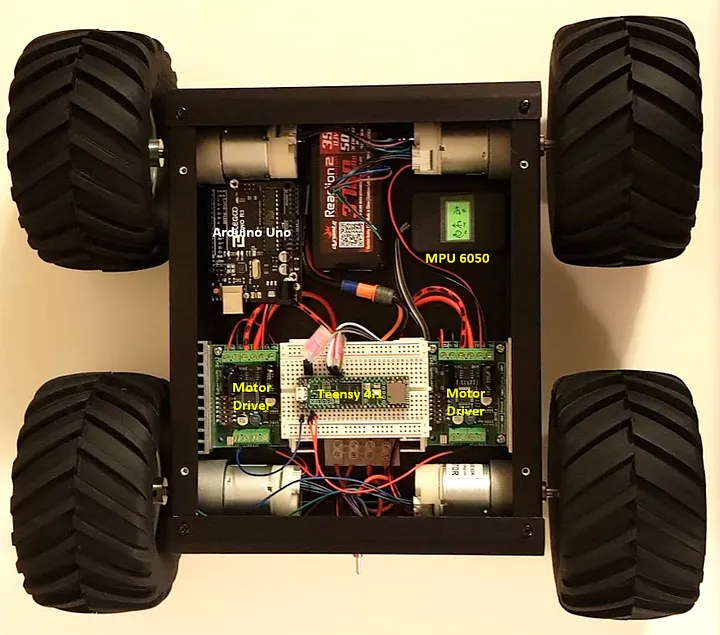
\includegraphics[width=0.88\linewidth]{figures/photos/rudra_chassis_top.png}
\caption{RUDRA chassis and deck layout reference from the engineering asset set.}
\end{figure}

For a 4WD skid-steer/differential rover, the ideal kinematic model is still the differential-drive model:
\begin{align}
v &= \frac{v_R+v_L}{2},\\
\omega &= \frac{v_R-v_L}{b},
\end{align}
where \(v\) is forward velocity, \(\omega\) is yaw rate, \(v_R\) and \(v_L\) are right and left side linear wheel velocities, and \(b\) is the wheelbase/track-width term used by the controller.  Real skid steer also includes scrub and slip, so odometry must be treated as a measured estimate, not ground truth.

\section{RUDRAv4 battery architecture}
RUDRAv4 uses two battery domains:

\begin{table}[h]
\centering
\caption{Battery domains used by RUDRAv4.}
\begin{tabularx}{\linewidth}{p{0.18\linewidth}p{0.27\linewidth}p{0.23\linewidth}Y}
\toprule
Domain & Pack & Nominal voltage & Purpose \\
\midrule
Motor power & Dynamite Reaction 2, 3S, \SI{11.1}{V}, 50C, \SI{41.07}{Wh} & \SI{11.1}{V} & Feeds Sabertooth motor drivers and drive motors. \\
NUC power & OVONIC, \SI{1550}{mAh}, 100C, 4S1P, \SI{14.8}{V}, \SI{22.94}{Wh} & \SI{14.8}{V} & Feeds Mini-Box DCDC-USB, which regulates to the NUC 19 V class input. \\
\bottomrule
\end{tabularx}
\end{table}

\begin{designbox}{Corrected OVONIC pack capacity}
The NUC battery is \SI{1550}{mAh}.  At \SI{14.8}{V} nominal, the stated pack energy is consistent: \(1.55\,\mathrm{Ah}\times14.8\,\mathrm{V}=\SI{22.94}{Wh}\).  Use the label value and measured runtime for operating decisions.
\end{designbox}

\section{Battery calculations}
For a LiPo pack:
\begin{equation}
E_{Wh}=V_{nominal} \times C_{Ah}.
\end{equation}

For the motor pack:
\begin{equation}
C_{Ah}=\frac{41.07}{11.1}=\SI{3.70}{Ah}.
\end{equation}

For the NUC pack as stated by capacity and nominal voltage:
\begin{equation}
E_{Wh}=14.8 \times 1.55=\SI{22.94}{Wh}.
\end{equation}

The approximate runtime is:
\begin{equation}
t_{hr}=\frac{E_{Wh}\eta}{P_{load}}.
\end{equation}

\begin{center}
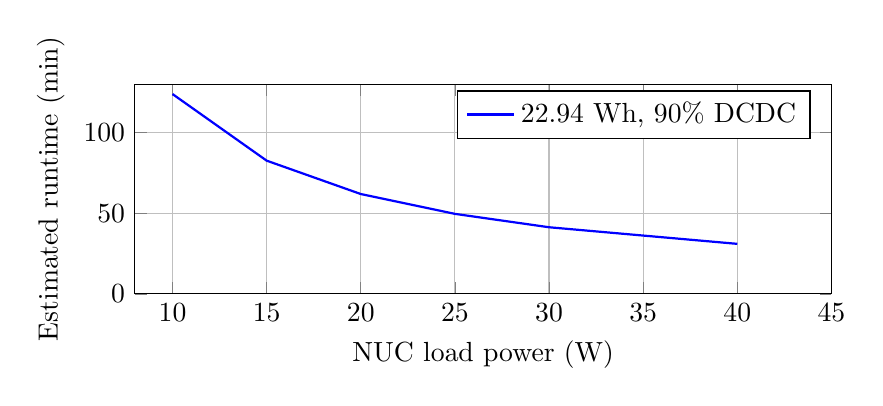
\begin{tikzpicture}
\begin{axis}[
  width=0.86\linewidth,
  height=0.35\linewidth,
  xlabel={NUC load power (W)},
  ylabel={Estimated runtime (min)},
  xmin=8,xmax=45,
  ymin=0,ymax=130,
  grid=both,
  legend pos=north east]
\addplot+[mark=none,thick] coordinates {(10,123.9) (15,82.6) (20,61.9) (25,49.6) (30,41.3) (40,31.0)};
\addlegendentry{22.94 Wh, 90\% DCDC}
\end{axis}
\end{tikzpicture}
\end{center}

The plot shows why the NUC battery should be monitored.  A small 4S pack can boot and run the NUC, but runtime depends strongly on CPU load, LiDAR/USB load, Wi-Fi, and DCDC efficiency.

\section{C-rating caution}
Theoretical discharge current from C-rating is:
\begin{equation}
I_{max,theory}=C_{rating} \times C_{Ah}.
\end{equation}

For the motor battery this gives \(50\times3.70=\SI{185}{A}\).  For the NUC battery using \SI{1.55}{Ah}, it gives \(100\times1.55=\SI{155}{A}\).  These values are marketing/pack capability indicators, not a reason to omit fuses, wire sizing, connector checks, or thermal checks.  The robot should be designed around measured current, connector limits, wiring gauge, and safe fuse ratings.

\section{Physical wiring and BOM reference}
The full wiring image from the RUDRA article remains valuable as the physical architecture reference.

\begin{figure}[h]
\centering
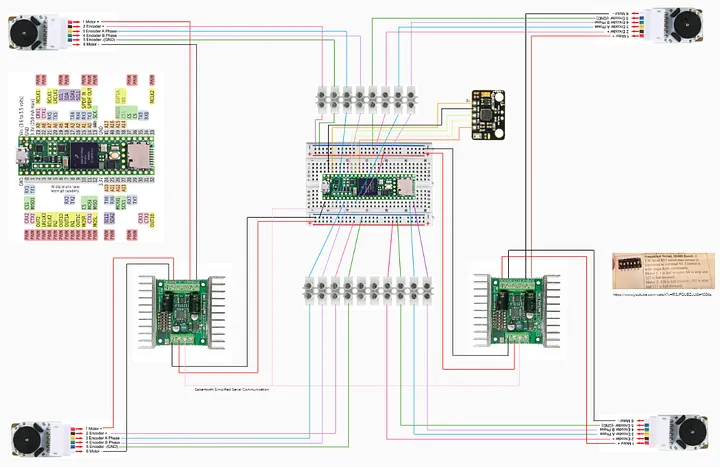
\includegraphics[width=0.96\linewidth]{figures/photos/rudra_wiring_detailed_full.png}
\caption{Detailed RUDRA base wiring reference: Teensy, Sabertooths, motors, IMU, encoder wiring, and power distribution.}
\end{figure}

The attached BOM screenshot is preserved below as a visual procurement reference.  It should not replace a version-controlled BOM file, but it is useful in the manual because it shows the real component stack used during the RUDRA build.

\begin{figure}[h]
\centering
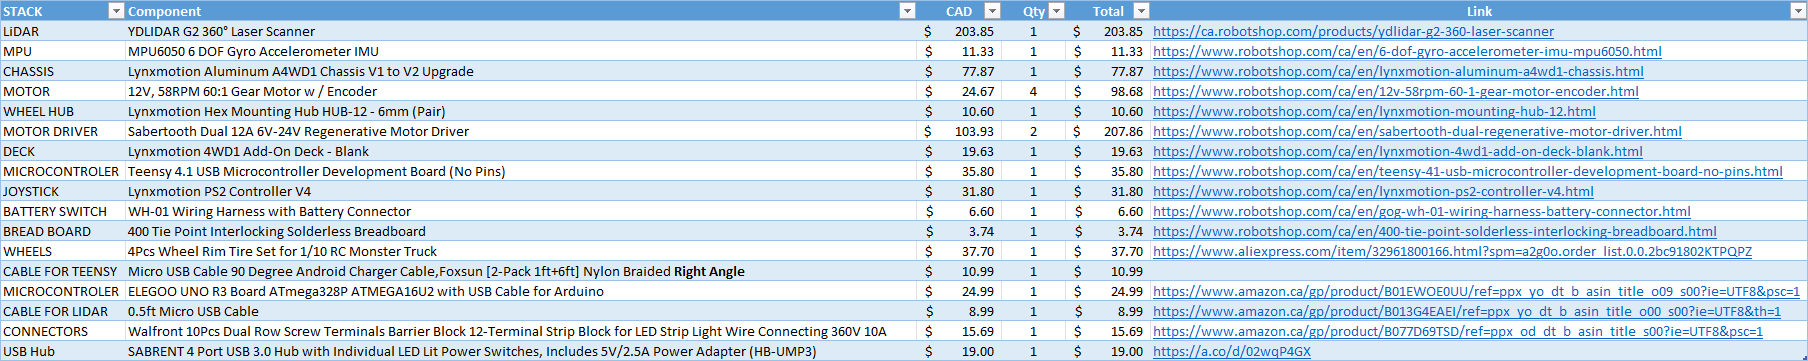
\includegraphics[width=0.96\linewidth]{figures/photos/rudra_bom_screenshot.png}
\caption{RUDRA hardware BOM screenshot supplied with this revision.  Keep the spreadsheet/source BOM under version control for exact part numbers, quantities, prices, and links.}
\end{figure}

\section{Mechanical integration notes}
\begin{itemize}
  \item Mount the NUC so the barrel connector and USB cables have strain relief.
  \item Keep the DCDC-USB and NUC power wiring away from the Sabertooth motor output wiring where practical.
  \item Route encoder and IMU signal wiring away from high-current motor leads.
  \item Secure LiPo packs mechanically; do not let them move during a sudden stop.
  \item Do not charge LiPo packs while installed inside a closed robot deck.
  \item Put an inline fuse or switch in the motor battery path and a separate accessible disconnect for the NUC rail.
\end{itemize}

\section{Verification before closing the deck}
\begin{enumerate}
  \item All grounds that must be common are common; power domains remain intentionally separated where required.
  \item Motor battery powers only the motor side.
  \item NUC battery powers the DCDC-USB input only.
  \item DCDC-USB output is verified before connecting to the NUC.
  \item USB cables are data-capable, not charge-only.
  \item \cmd{bash scripts/list_serial.sh} shows Uno, Teensy, and YDLIDAR adapter.
  \item \topic{/rudra/nuc_battery} publishes when the DCDC monitor is launched.
\end{enumerate}
